\documentclass{beamer}
% \documentclass[handout]{beamer}

\usepackage[sfdefault]{AlegreyaSans}

\usepackage{inconsolata} % IMPORTANTE CAMBIA TIPOGRAFIA MONO A ALGO CRISTIANO

\usepackage{multicol}
\usepackage{multirow}
\usepackage[spanish]{babel}
\usepackage[utf8]{inputenc}

% \usetheme{Warsaw}
\usetheme{Pittsburgh}
% \usetheme{boxes}

\usecolortheme[rgb={1,0.48,0.0}]{structure}%divido los RGB por 252
\setbeamercolor{block title}{fg=white,bg=verdeuca}
\xdefinecolor{verdeuca}{rgb}{0.0,0.48,0.54}
\xdefinecolor{naranjauca}{rgb}{1,0.48,0.0}
\setbeamercolor{palette quaternary}{fg=white,bg=verdeuca}
\xdefinecolor{energia}{rgb}{0.98,0.68,0.24}

\setbeamertemplate{title page}[default][colsep=-4bp, rounded=true] % borra sombra en titulo general
\setbeamertemplate{frametitle}[default][colsep=-2bp, shadow=false] % borra sombra en titulo del frame

% \usepackage[shortlabels]{enumitem} % para tener items enumerados con circulos (remplaza \usepackage{enumerate})
\usepackage{enumerate}
\usepackage{color}
\usepackage{xcolor}
\usepackage[absolute,overlay]{textpos}
  \setlength{\TPHorizModule}{1mm}
  \setlength{\TPVertModule}{1mm}
\usepackage{framed}
\usepackage{mfirstuc} % para poner en mayusculas la primer letra
\usepackage{xspace} % para crear espacios en comandos 
\usepackage[binary-units]{siunitx} % para tener unidades SI

\usepackage{listings}
\definecolor{verbgray}{gray}{0.9}
\lstnewenvironment{code}{
\lstset{backgroundcolor=\color{verbgray},
frame=single,
framerule=0pt,
basicstyle=\ttfamily,
columns=fullflexible}}{}

\setbeamertemplate{navigation symbols}{} %remove navigation symbols

% % % TABLAS
\newcolumntype{P}[1]{>{\centering\arraybackslash}p{#1}}
\newcolumntype{C}[1]{>{\centering\arraybackslash}m{#1}}
\newcolumntype{R}[1]{>{\raggedleft\arraybackslash}m{#1}}

% % % COLORES
\definecolor{AzulClaro}{rgb}{.31,.506,.741}
\definecolor{GRIS}{gray}{0.8}
\newcommand{\T}[0]{{\cellcolor[gray]{.8}}}

% % % RENOMBRES
\newcommand{\tab}[0]{\hspace{15pt}}
\newcommand{\gemCinco}[0]{\texttt{gem5}\xspace} % \titlecap{\gemCinco}
\newcommand{\McPAT}[0]{\texttt{McPAT}\xspace}
\newcommand{\Mth}[0]{\textsl{Mth}\xspace}
\newcommand{\XML}[0]{\texttt{XML}\xspace}

% % % COLORES DE BLOCKES
\setbeamercolor{block body}{fg=black, bg=black!10}
\setbeamercolor{block title}{fg=black, bg=black!20}

% Zoolander: Para niños que no saben leer bien y quieren aprender a hacer otras cosas buenas también
\title[]{\large \textsc{Charla para estudiantes que saben usar la computadora\\ bien y quieren aprender a hacer otras cosas bien también}}
\author[D. Gonz\'alez M\'arquez, M. Geier]{
  \footnotesize{David Alejandro Gonz\'alez M\'arquez}\\
  \footnotesize{Maximiliano Geier}
}
  
\date{}

\begin{document}

\begin{frame}[plain]
\vspace{2cm}
  \titlepage
\end{frame}

\begin{frame}[fragile]
    \frametitle{Charlas para estudiantes que saben usar la computadora\\ bien y quieren aprender a hacer otras cosas bien también}
    \begin{itemize}
    \setlength\itemsep{1cm}
    \Large
    \item[] \only<1>{\textcolor{naranjauca}{Charla 01} - Procesamiento de texto}
            \only<2>{\textcolor{naranjauca}{Charla 01} - Procesamiento de texto}
    \item[] \only<1>{\textcolor{naranjauca}{Charla 02} - Sistema linux y redes}
            \only<2>{\textcolor{black!40  }{Charla 02  - Sistema linux y redes}}
    \item[] \only<1>{\textcolor{naranjauca}{Charla 03} - Compilaci\'on y procesos}
            \only<2>{\textcolor{black!40  }{Charla 03  - Compilaci\'on y procesos}}
    \end{itemize}
\end{frame}

\begin{frame}[fragile]
    \frametitle{Charla 01 \textcolor{black}{- Procesamiento de texto}}
    Objetivo
    \begin{itemize}
    \setlength\itemsep{0.5cm}
    \item Enseñar comandos y combinaciones de comandos.
    \item Luego de la charla se espera que busquen ejemplos.
    \item Es una referencia \emph{quick and dirty}.
    \end{itemize}
    \vspace{1cm}
    Público 
    \begin{itemize} 
    \setlength\itemsep{0.5cm}
    \item Cualquiera que quiera aprender a procesar texto eficientemente con herramientas simples.
    \end{itemize}
\end{frame}

\begin{frame}[fragile]
    \frametitle{¿Por qué aprender esto?}
    \begin{textblock}{20}(20,10)
    \only<2->{
\includegraphics[scale=0.95]{img/antesydespuesreferencias.pdf}}
    \end{textblock}
    \begin{textblock}{20}(7,26)
    \only<3->{\includegraphics[scale=0.95]{img/antesydespues-layer1.pdf}}
    \end{textblock}
    \begin{textblock}{20}(7,26)
    \only<4->{\includegraphics[scale=0.95]{img/antesydespues-layer2.pdf}}
    \end{textblock}
    \begin{textblock}{20}(7,26)
    \only<5->{\includegraphics[scale=0.95]{img/antesydespues-layer3.pdf}}
    \end{textblock}
    \begin{textblock}{20}(7,26)
    \only<6->{\includegraphics[scale=0.95]{img/antesydespues-layer4.pdf}}
    \end{textblock}
    \begin{textblock}{120}(7,60)
    \begin{itemize}
    \item<7-> Usar bien los comandos requiere \textbf{entrenamiento} y \textbf{práctica}.
    \item<8-> Si después de está charla no aplican lo aprendido en su trabajo $\cdots$
    \end{itemize}
    \end{textblock}
    \begin{textblock}{120}(0,70)
    \begin{center}
    \only<9->{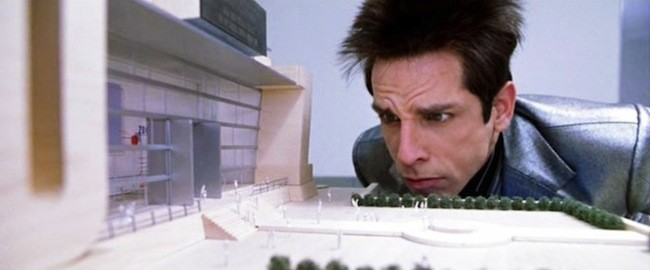
\includegraphics[scale=0.22]{img/zoolander.jpg}}
    \end{center}
    \end{textblock}  
    % - Requiere entrenamiento y practica
    %       antes     |-----------------------------|
    %       despues   |----buscar/google----|hacer|
    %       entrenado |buscar|hacer|
    %       sabe      |hacer|
\end{frame}

% \colorbox{verdeuca}{ \small \textcolor{white}{ asdasdasde } }\\

\begin{frame}[fragile,t]
    \frametitle{Commando \texttt{echo}}
    \begin{block}{\vspace*{-3ex}}
    \texttt{\$}\verb: echo "hello world":
    \vspace*{0.5ex}
    \end{block}
    \begin{itemize}
    \item[-] Toma un texto como parámetro (``\texttt{hello world}'').
    \item[-] Imprime en la salida estándar (\verb|stdout|) el parámetro.
    \end{itemize}
    \vspace{2.5cm}
    \pause
    \begin{block}{\vspace*{-3ex}}
    \texttt{\$}\verb: echo "hello world":\\
    \verb:hello world:
    \vspace*{0.5ex}
    \end{block}
    \begin{textblock}{100}(20,38)
    \begin{center}
    \only<2->{\includegraphics[scale=0.65]{img/programas-layer1.pdf}}
    \end{center}
    \end{textblock}
\end{frame}

\begin{frame}[fragile,t]
    \frametitle{Commando \texttt{wc} y operador \texttt{|}}
    \begin{block}{\vspace*{-3ex}}
    \texttt{\$}\verb: echo "hello world" | wc:
    \vspace*{0.5ex}
    \end{block}
    \begin{itemize}
    \item[-] El operador ``\verb.|.'' (pipe) conecta una salida con una entrada.
    \item[-] El programa ``\verb|wc|'' cuenta líneas, palabras y caracteres.
    \item[-] Toma por su entrada estándar (\verb|stdin|) el resultado de ``\verb|echo|''.
    \end{itemize}
    \vspace{2.5cm}
    \pause
    \begin{block}{\vspace*{-3ex}}
    \texttt{\$}\verb: echo "hello world" | wc:\\
    \verb:       1       2      12:
    \vspace*{0.5ex}
    \end{block}
    \begin{textblock}{100}(20,44)
    \begin{center}
    \only<2->{\includegraphics[scale=0.65]{img/programas-layer2.pdf}}
    \end{center}
    \end{textblock}
\end{frame}

\begin{frame}[fragile,t]
    \frametitle{Commando \texttt{cat}}
    \begin{block}{\vspace*{-3ex}}
    \texttt{\$}\verb: cat sarasa.txt:
    \vspace*{0.5ex}
    \end{block}
    \begin{itemize}
    \item[-] El programa ``\verb|cat|'' lee un archivo y lo imprime por \verb|stdout|.
    \item[-] Además de \verb|stdout| los programas pueden generar \verb|stderr| (salida de error).
    \end{itemize}
    \vspace{2.5cm}
    \pause
    \begin{block}{\vspace*{-3ex}}
    \texttt{\$}\verb: cat sarasa.txt:\\
    \verb;cat: sarasa.txt: No such file or directory;
    \vspace*{0.5ex}
    \end{block}
    \begin{textblock}{100}(20,44)
    \begin{center}
    \only<2->{\includegraphics[scale=0.65]{img/programas-layer3.pdf}}
    \end{center}
    \end{textblock}
\end{frame}

\begin{frame}[fragile,t]
    \frametitle{Operador \texttt{>}}
    \begin{block}{\vspace*{-3ex}}
    \texttt{\$}\verb: echo "hello world" > a.txt:
    \vspace*{0.5ex}
    \end{block}
    \begin{itemize}
    \item[-] El operador ``\verb|>|'' permite redireccionar la salida a un archivo.
    \end{itemize}
    \vspace{2.5cm}
    \pause
    \begin{block}{\vspace*{-3ex}}
    \texttt{\$}\verb: echo "hello world" > a.txt:\\
    \vspace{0.2cm}
    \texttt{\$}\verb: cat a.txt:\\
    \verb:hello world:
    \vspace*{0.5ex}
    \end{block}
    \begin{textblock}{100}(20,35)
    \begin{center}
    \only<2->{\includegraphics[scale=0.65]{img/programas-layer4.pdf}}
    \end{center}
    \end{textblock}
\end{frame}

\begin{frame}[fragile,t]
    \frametitle{Operador \texttt{>>}}
    \begin{block}{\vspace*{-3ex}}
    \texttt{\$}\verb: cat a.txt >> file.txt:
    \vspace*{0.5ex}
    \end{block}
    \begin{itemize}
    \item[-] El operador ``\verb|>>|'' permite redireccionar la salida y la concatena a un archivo.
    \end{itemize}
    \vspace{1.8cm}
    \pause
    \begin{block}{\vspace*{-3ex}}
    \texttt{\$}\verb: cat file.txt:\\
    \verb:texto cualquiera:\\
    \vspace{0.2cm}
    \texttt{\$}\verb: cat a.txt >> file.txt:\\
    \texttt{\$}\verb: cat file.txt:\\
    \verb:texto cualquiera:\\
    \verb:hello world:
    \vspace*{0.5ex}
    \end{block}
    \begin{textblock}{100}(20,33)
    \begin{center}
    \only<2->{\includegraphics[scale=0.65]{img/programas-layer5.pdf}}
    \end{center}
    \end{textblock}
\end{frame}

\begin{frame}[fragile,t]
    \frametitle{Operador \texttt{\&>}}
    \begin{block}{\vspace*{-3ex}}
    \texttt{\$}\verb: cat sarasa.txt &> a.txt:
    \vspace*{0.5ex}
    \end{block}
    \begin{itemize}
    \item[-] El operador ``\verb|&>|'' permite redireccionar \verb|stdout| y \verb|stderr| a un archivo.
    \end{itemize}
    \vspace{1.8cm}
    \pause
    \begin{block}{\vspace*{-3ex}}
    \texttt{\$}\verb: cat sarasa.txt > a.txt:\\
    \verb;cat: sarasa.txt: No such file or directory;\\
    \vspace{0.2cm}
    \texttt{\$}\verb: cat sarasa.txt &> a.txt:\\
    \texttt{\$}\verb: cat a.txt:\\
    \verb;cat: sarasa.txt: No such file or directory;
    \vspace*{0.5ex}
    \end{block}
    \begin{textblock}{100}(35,35)
    \begin{center}
    \only<2->{\includegraphics[scale=0.65]{img/programas-layer6.pdf}}
    \end{center}
    \end{textblock}
\end{frame}

\begin{frame}[fragile,t]
    \frametitle{Commando \texttt{grep}}
    \begin{block}{\vspace*{-3ex}}
    \texttt{\$}\verb: grep "hello" file.txt:
    \vspace*{0.5ex}
    \end{block}
    \begin{itemize}
    \item[-] El programa \verb|grep| busca línea por línea el texto \verb|hello| en el archivo \verb|file.txt|.
    \end{itemize}
    \vspace{1.8cm}
    \pause
    \begin{block}{\vspace*{-3ex}}
    \texttt{\$}\verb: cat file.txt:\\
    \verb;red = rojo;\\
    \verb;hola = hello;\\
    \verb;cat = gato;\\
    \vspace{0.2cm}
    \texttt{\$}\verb: grep "hello" file.txt:\\
    \verb;hola = hello;\\
    \vspace*{0.5ex}
    \end{block}
    \begin{textblock}{100}(35,34)
    \begin{center}
    \only<2->{\includegraphics[scale=0.65]{img/programas-layer7.pdf}}
    \end{center}
    \end{textblock}
\end{frame}

\begin{frame}[fragile,t]
    \frametitle{Commando \texttt{grep}}
    \begin{block}{\vspace*{-3ex}}
    \texttt{\$}\verb: cat file.txt | grep "hello":
    \vspace*{0.5ex}
    \end{block}
    \vspace{-0.2cm}
    \begin{itemize}
    \item[-] Otra opci\'on es imprimir en \verb|stdout| y luego redireccionarlo a \verb|grep|.
    \end{itemize}
    \vspace{1.8cm}
    \pause
    \begin{block}{\vspace*{-3ex}}
    \texttt{\$}\verb: cat file.txt:\\
    \verb;red = rojo;\\
    \verb;hola = hello;\\
    \verb;cat = gato;\\
    \vspace{0.2cm}
    \texttt{\$}\verb: cat file.txt | grep "hello":\\
    \verb;hola = hello;\\
    \vspace*{0.5ex}
    \end{block}
    \begin{textblock}{100}(20,29)
    \begin{center}
    \only<2->{\includegraphics[scale=0.65]{img/programas-layer8.pdf}}
    \end{center}
    \end{textblock}
\end{frame}

\begin{frame}[fragile,t]
    \frametitle{Commando \texttt{grep}}
    \verb|grep| además soporta expresiones regulares:\\
    \vspace{0.2cm}
    \begin{itemize}
    \item[-] Ejemplos
    \begin{itemize}
    \item[$\cdot$] ``\verb|^____|'' = busca al comienzo de la línea.
    \item[$\cdot$] ``\verb|____$|'' = busca al final de la línea.
    \item[$\cdot$] ``\verb|__.__|'' = un caracter cualquiera.
    \item[$\cdot$] ``\verb|__.*_|'' = un conjunto de caracteres cualquiera.
    \end{itemize}
    \vspace{0.2cm}
    \item[-] Otros parámetros:
    \item[$\cdot$] \verb|-i| = insensible.
    \item[$\cdot$] \verb|-v| = inverso.
    \item[$\cdot$] \verb|-r| = recursivo.
    \item[$\cdot$] \verb|-A |$n$ = imprime n líneas arriba del encontrado.
    \item[$\cdot$] \verb|-B |$n$ = imprime n líneas debajo del encontrado.
    \item[$\cdot$] \verb|-C |$n$ = imprime n líneas arriba y abajo del encontrado.
    \end{itemize}
\end{frame}

\begin{frame}[fragile,t]
    \frametitle{Commando \texttt{sed}}
    \begin{block}{\vspace*{-3ex}}
    \texttt{\$}\verb: sed 's/__1__/__2__/g' file.txt:
    \vspace*{0.5ex}
    \end{block}
    \begin{itemize}
    \item[-] Remplaza todas las apariciones de ``\verb|__1__|'' por ``\verb|__2__|'' en file.txt\\ e imprime el resultado en la \texttt{stdout}.
    \item[-] ``\verb|g|'' indica que remplaza todas las apariciones.
    \end{itemize}
    \vspace{2cm}
    \pause
    \begin{block}{\vspace*{-3ex}}
    \texttt{\$}\verb: sed -i 's/__1__/__2__/g' file.txt:
    \vspace*{0.5ex}
    \end{block}
    \begin{itemize}
    \item[-] La opci\'on ``\verb|-i|'' modifica el archivo \verb|file.txt|.
    \end{itemize}
    \begin{textblock}{100}(20,42)
    \begin{center}
    \only<2->{\includegraphics[scale=0.65]{img/programas-layer9.pdf}}
    \end{center}
    \end{textblock}
\end{frame}

\begin{frame}[fragile,t]
    \frametitle{Commando \texttt{awk}}
    \begin{block}{\vspace*{-3ex}}
    \texttt{\$}\verb: cat file.txt | awk '{print $3}':
    \vspace*{0.5ex}
    \end{block}
    \begin{itemize}
    \item[-] ``\verb|awk|'' es un lenguaje de procesamiento de texto.
    \item[-] \emph{tokeniza} cada línea y ejecuta el programa indicado.
    \item[-] usa como separador espacios o tabs.
    \item[-] el operador ``\verb|$i|'' se remplaza el i-ésimo texto tokenizado.
    \end{itemize}
    \vspace{2.3cm}
    \pause
    \textcolor{naranjauca}{Ejemplo:}\\
    \verb;Estúpido y sensual Flanders!;\\
    \verb;$1 = "Estúpido", $2 = "y" $3 = "sensual", $4 = "Flanders!";\\
    \begin{textblock}{100}(20,50)
    \begin{center}
    \only<2->{\includegraphics[scale=0.65]{img/programas-layer10.pdf}}
    \end{center}
    \end{textblock}
\end{frame}

\begin{frame}[fragile,t]
    \frametitle{Commando \texttt{awk}}
    \begin{block}{\vspace*{-3ex}}
    \texttt{\$}\verb: cat file.txt:\\
    \verb:Wenquan  China    5.000:\\
    \verb:Potosí   Bolivia  4.090:\\
    \verb:Oruro    Bolivia  3.706:\\
    \verb:Lhasa    China    3.650:\\
    \verb:Cuzco    Perú     3.399:
    \vspace*{0.5ex}
    \end{block}
    \vspace{0.2cm}
    \begin{block}{\vspace*{-3ex}}
    \texttt{\$}\verb: cat file.txt | awk '{print $3}':\\
    \verb:5.000:\\
    \verb:4.090:\\
    \verb:3.706:\\
    \verb:3.650:\\
    \verb:3.399:
    \vspace*{0.5ex}
    \end{block}
\end{frame}

\begin{frame}[fragile,t]
    \frametitle{Commando \texttt{awk}}
    \begin{block}{\vspace*{-3ex}}
    \texttt{\$}\verb: cat file.txt | awk -F "." '{print $3}':
    \vspace*{0.5ex}
    \end{block}
    \begin{itemize}
    \item[-] El parametro ``\verb|-F|'' indica el separador utilizado.
    \end{itemize}
    \pause
    \vspace{-0.5cm}
    \begin{block}{\vspace*{-3ex}}
    \small
    \texttt{\$}\verb: cat autobots.txt:\\
    \verb:Name.Alternate modes.Rank.Function:\\
    \verb:Optimus Prime.Peterbilt flat-nosed.10.Autobot Leader:\\
    \verb:Bumblebee.Volkswagen Beetle.7.Espionage:\\
    % \verb:Trailbreaker.1986 Toyota Hilux 4x4 Camper.7.Defensive Strategist:\\
    \verb:Windcharger.Pontiac Fire Bird Trans Am.5.Warrior:\\
    \verb:Outback.Land Rover.4.Administrative Assistant:\\
    \vspace{0.2cm}
    \texttt{\$}\verb: cat autobots.txt | awk -F "." '{print $3}':\\
    \verb:Rank:\\
    \verb:10:\\
    \verb:7:\\
    % \verb:7:\\
    \verb:5:\\
    \verb:4:\\
    \vspace*{0.5ex}
    \end{block}
\end{frame}

\begin{frame}[fragile,t]
    \frametitle{Commando \texttt{sort} y \texttt{uniq}}
    \vspace{-0.5cm}
    \begin{block}{\vspace*{-3ex}}
    \texttt{\$}\verb: cat file.txt | sort | uniq:
    \vspace*{0.5ex}
    \end{block}
    \vspace{-0.2cm}
    \begin{itemize}
    \item[-] ``\verb|sort|'' ordena lexicográficamente las líneas.
    \item[-] ``\verb|uniq|'' imprime una línea si es distinta a la anterior.
    \end{itemize}
    \begin{textblock}{100}(3,31)
    \begin{center}
    \only<2->{\includegraphics[scale=0.65]{img/programas-layer11.pdf}}
    \end{center}
    \end{textblock}
    \begin{textblock}{35}(7,57)
    \begin{block}<only@3->{\vspace*{-3ex}}
    \scriptsize
    \verb:Japan:\\
    \verb:Russia:\\
    \verb:Japan:\\
    \verb:Egypt:\\
    \verb:South Korea:\\
    \verb:Egypt:\\
    \verb:Bangladesh:\\
    \verb:South Korea:\\
    \verb:Mexico:\\
    \verb:Bangladesh:\\
    \vspace*{0.5ex}
    \end{block}
    \end{textblock}
    \begin{textblock}{35}(37,60)
    \only<3->{file}
    \end{textblock}
    \begin{textblock}{35}(47,57)
    \begin{block}<only@3->{\vspace*{-3ex}}
    \scriptsize
    \verb:Bangladesh:\\
    \verb:Bangladesh:\\
    \verb:Egypt:\\
    \verb:Egypt:\\
    \verb:Japan:\\
    \verb:Japan:\\
    \verb:Mexico:\\
    \verb:Russia:\\
    \verb:South Korea:\\
    \verb:South Korea:\\
    \vspace*{0.5ex}
    \end{block}
    \end{textblock}
    \begin{textblock}{35}(76,60)
    \only<3->{sort}
    \end{textblock}
    \begin{textblock}{35}(87,57)
    \begin{block}<only@3->{\vspace*{-3ex}}
    \scriptsize
    \verb:Bangladesh:\\
    \verb:Egypt:\\
    \verb:Japan:\\
    \verb:Mexico:\\
    \verb:Russia:\\
    \verb:South Korea:\\
    \vspace*{0.5ex}
    \end{block}
    \end{textblock}
    \begin{textblock}{35}(115,60)
    \only<3->{uniq}
    \end{textblock}
\end{frame}

\begin{frame}[fragile,t]
    \frametitle{Commando \texttt{sort} y \texttt{uniq}}
    \vspace{-0.5cm}
    \begin{block}{\vspace*{-3ex}}
    \texttt{\$}\verb: cat file.txt | sort -n | uniq -c:
    \vspace*{0.5ex}
    \end{block}
    \vspace{-0.2cm}
    \begin{itemize}
    \item[-] ``\verb|-n|'' ordena numéricamente usando el primer dato como número.
    \item[-] ``\verb|-c|'' indica la cantidad de líneas que fueron no impresas.
    \end{itemize}
    \begin{textblock}{100}(3,30)
    \begin{center}
    \only<2->{\includegraphics[scale=0.65]{img/programas-layer12.pdf}}
    \end{center}
    \end{textblock}
    \begin{textblock}{35}(7,57)
    \begin{block}<only@3->{\vspace*{-3ex}}
    \scriptsize
    \verb:123 sarasa:\\
    \verb:99:\\
    \verb:123 SARASA:\\
    \verb:9999:\\
    \verb:99:\\
    \verb:313:\\
    \verb:123 sarasa:\\
    \verb:9999:\\
    \verb:213:\\
    \verb:9999:
    \vspace*{0.5ex}
    \end{block}
    \end{textblock}
    \begin{textblock}{35}(37,60)
    \only<3->{file}
    \end{textblock}
    \begin{textblock}{35}(47,57)
    \begin{block}<only@3->{\vspace*{-3ex}}
    \scriptsize
    \verb:99:\\
    \verb:99:\\
    \verb:123 sarasa:\\
    \verb:123 sarasa:\\
    \verb:123 SARASA:\\
    \verb:213:\\
    \verb:313:\\
    \verb:9999:\\
    \verb:9999:\\
    \verb:9999:
    \vspace*{0.5ex}
    \end{block}
    \end{textblock}
    \begin{textblock}{35}(76,60)
    \only<3->{sort}
    \end{textblock}
    \begin{textblock}{35}(87,57)
    \begin{block}<only@3->{\vspace*{-3ex}}
    \scriptsize
    \verb:      2 99:\\
    \verb:      2 123 sarasa:\\
    \verb:      1 123 SARASA:\\
    \verb:      1 213:\\
    \verb:      1 313:\\
    \verb:      3 9999:
    \vspace*{0.5ex}
    \end{block}
    \end{textblock}
    \begin{textblock}{35}(115,60)
    \only<3->{uniq}
    \end{textblock}
\end{frame}

\begin{frame}[fragile,t]
    \frametitle{Commando \texttt{find}}
    \begin{block}{\vspace*{-3ex}}
    \texttt{\$}\verb: find:
    \vspace*{0.5ex}
    \end{block}
    \begin{itemize}
    \item[-] Imprime todos los nombres de archivos/carpetas recursivamente desde la carpeta actual.
    \end{itemize}
    \begin{textblock}{100}(10,45)
    \begin{center}
    \only<2->{\includegraphics[scale=0.65]{img/programas-layer13.pdf}}
    \end{center}
    \end{textblock}
    \begin{textblock}{50}(67,33)
    \begin{block}<only@3->{\vspace*{-3ex}}
    \small
    \verb:.:\\
    \verb:./results.txt:\\
    \verb:./files:\\
    \verb:./files/other:\\
    \verb:./files/other/file.txt:\\
    \verb:./files/file.txt:\\
    \verb:./colums.dat:\\
    \verb:./country.txt:\\
    \verb:./sources.list:\\
    \verb:./numbers.txt:\\
    \verb:./names.txt:\\
    \verb:./autobots.txt:\\
    \verb:./hosts:
    \vspace*{0.5ex}
    \end{block}
    \end{textblock} 
\end{frame}

\begin{frame}[fragile,t]
    \frametitle{Commando \texttt{find}}
    \begin{block}{\vspace*{-3ex}}
    \texttt{\$}\verb: find -name '*.txt' -type f:
    \vspace*{0.5ex}
    \end{block}
    \begin{itemize}
    \item[-] Imprime solamente los archivos cuyo nombre termina con ``\verb|.txt|''.
    \end{itemize}
    \begin{textblock}{100}(10,45)
    \begin{center}
    \only<1->{\includegraphics[scale=0.65]{img/programas-layer13.pdf}}
    \end{center}
    \end{textblock}
    \begin{textblock}{50}(67,40)
    \only<2->{Ejemplo:} \vspace{-0.5cm}
    \begin{block}<only@2->{\vspace*{-3ex}}
    \small
    \verb:./results.txt:\\
    \verb:./files/other/file.txt:\\
    \verb:./files/file.txt:\\
    \verb:./country.txt:\\
    \verb:./numbers.txt:\\
    \verb:./names.txt:\\
    \verb:./autobots.txt:\\
    \vspace*{0.5ex}
    \end{block}
    \end{textblock}
\end{frame}

\begin{frame}[fragile,t]
    \frametitle{Commando \texttt{find}}
    \begin{block}{\vspace*{-3ex}}
    \texttt{\$}\verb: find -name '*.txt' -type f -exec wc -l {} \;:
    \vspace*{0.5ex}
    \end{block}
    \begin{itemize}
    \item[-] Por cada archivo terminado en ``\verb|.txt|'' ejecuta ``\verb|wc -l|''. Esto cuenta la cantidad líneas de cada archivo.
    \end{itemize}
    \begin{textblock}{100}(10,45)
    \begin{center}
    \only<1->{\includegraphics[scale=0.65]{img/programas-layer13.pdf}}
    \end{center}
    \end{textblock}
    \begin{textblock}{50}(67,45)
    \only<2->{Ejemplo:} \vspace{-0.5cm}
    \begin{block}<only@2->{\vspace*{-3ex}}
    \small
    \verb:19 ./results.txt:\\
    \verb:1 ./files/other/file.txt:\\
    \verb:1 ./files/file.txt:\\
    \verb:10 ./country.txt:\\
    \verb:10 ./numbers.txt:\\
    \verb:51 ./names.txt:\\
    \verb:6 ./autobots.txt:
    \vspace*{0.5ex}
    \end{block}
    \end{textblock}
\end{frame}

\begin{frame}[fragile,t]
    \frametitle{Commando \texttt{xargs}}
    \begin{block}{\vspace*{-3ex}}
    \texttt{\$}\verb: find -name '*.txt' -type f | xargs wc -l:
    \vspace*{0.5ex}
    \end{block}
    \begin{itemize}
    \item[-] \verb|xargs| toma varios archivos al mismo tiempo por \verb|stdin| y ejecuta el comando pasado por parámetro.
    \item[-] Esto concatena todos los archivos, y los pasa todos juntos a \verb|wc -l| (cuenta líneas totales).
    \end{itemize}
    \begin{textblock}{100}(2,55)
    \begin{center}
    \only<2->{\includegraphics[scale=0.65]{img/programas-layer15.pdf}}
    \end{center}
    \end{textblock}
    \begin{textblock}{36}(88,55)
    \only<3->{Ejemplo:} \vspace{-0.5cm}
    \begin{block}<only@3->{\vspace*{-3ex}}
    \scriptsize
    \verb:19 ./results.txt:\\
    \verb: 1 ./files/other/file.txt:\\
    \verb: 1 ./files/file.txt:\\
    \verb:10 ./country.txt:\\
    \verb:10 ./numbers.txt:\\
    \verb:51 ./names.txt:\\
    \verb: 6 ./autobots.txt:\\
    \verb:98 total:
    \vspace*{0.5ex}
    \end{block}
    \end{textblock}
\end{frame}

\begin{frame}[fragile,t]
    \frametitle{Commando \texttt{head}}
    \begin{block}{\vspace*{-3ex}}
    \texttt{\$}\verb: cat file.txt | head -n 5:
    \vspace*{0.5ex}
    \end{block}
    \begin{itemize}
    \item[-] Imprime las primeras 5 líneas de un archivo.
    \end{itemize}
    \begin{textblock}{100}(20,35)
    \begin{center}
    \only<2->{\includegraphics[scale=0.65]{img/programas-layer17.pdf}}
    \end{center}
    \end{textblock}
    \begin{textblock}{36}(20,65)
    \only<3->{Ejemplo:} \vspace{-0.5cm}
    \begin{block}<only@3->{\vspace*{-3ex}}
    \small
    \verb:Dots  Boxes:\\
    \verb:13    2134:\\
    \verb:4     4325:\\
    \verb:12    234:\\
    \verb:23    43:
    \vspace*{0.5ex}
    \end{block}
    \end{textblock}
\end{frame}

\begin{frame}[fragile,t]
    \frametitle{Commando \texttt{tail}}
    \begin{block}{\vspace*{-3ex}}
    \texttt{\$}\verb: cat columns.dat | tail -n 5:
    \vspace*{0.5ex}
    \end{block}
    \begin{itemize}
    \item[-] Imprime las últimas 5 líneas del archivo.
    \end{itemize}
    \begin{textblock}{100}(20,35)
    \begin{center}
    \only<2->{\includegraphics[scale=0.65]{img/programas-layer16.pdf}}
    \end{center}
    \end{textblock}
    \begin{textblock}{36}(20,65)
    \only<3->{Ejemplo:} \vspace{-0.5cm}
    \begin{block}<only@3->{\vspace*{-3ex}}
    \small
    \verb:463   56:\\
    \verb:4     795:\\
    \verb:75    2:\\
    \verb:632   690:\\
    \verb:46    78:
    \vspace*{0.5ex}
    \end{block}
    \end{textblock}
\end{frame}

\begin{frame}[fragile,t]
    \frametitle{Commando \texttt{tail}}
    \begin{block}{\vspace*{-3ex}}
    \texttt{\$}\verb: tail -f /var/log/syslog:
    \vspace*{0.5ex}
    \end{block}
    \begin{itemize}
    \item[-] Muestra las últimas líneas 10 líneas
    \item[-] Además, se queda esperando a que otro programa agregue nuevas líneas al mismo archivo para mostrarlas.
    \end{itemize}
    \begin{textblock}{100}(5,50)
    \begin{center}
    \only<2->{\includegraphics[scale=0.65]{img/programas-layer14.pdf}}
    \end{center}
    \end{textblock}
    \begin{textblock}{150}(55,47)
    \only<3->{Ejemplo:} \vspace{-0.5cm}
    \begin{block}<only@3->{\vspace*{-3ex}}
    \scriptsize
    \verb;May 12 00:53:54 faraday dhclient[14419]: XMT: Request on wlp2s0, interval 1070ms.;\\
    \verb;May 12 00:53:54 faraday NetworkManager[853]: <info>  [1557633234.1667] dhcp (wlp2s0):   domain search 'lan.';\\
    \verb;May 12 00:53:54 faraday NetworkManager[853]: <info>  [1557633234.1667] dhcp6 (wlp2s0): state changed unknown -> bound, event ID="00:22:11:ff|13234";\\
    \verb;May 12 00:53:56 faraday whoopsie[1556]: [00:53:56] online;\\
    \verb;May 12 00:53:56 faraday kdeconnectd.desktop[2511]: kdeconnect.core: Broadcasting identity packet;\\
    \verb;May 12 00:53:56 faraday kdeconnectd.desktop[2511]: kdeconnect.core: Starting client ssl (but I'm the server TCP socket);\\
    \verb;May 12 00:53:56 faraday kdeconnectd.desktop[2511]: kdeconnect.core: Socket succesfully stablished an SSL connection;\\
    \verb;May 12 00:53:56 faraday kdeconnectd.desktop[2511]: kdeconnect.core: It is a new device "david@belgrano";\\
    \verb;_;\\
    \vspace*{0.5ex}
    \end{block}
    \only<3->{
    \scriptsize \textcolor{naranjauca}{[tail espera que más caracteres se escriban en el archivo] }\\
    \scriptsize Se termina el programa con \texttt{Control + C}
    }
    \end{textblock}
\end{frame}

\begin{frame}[fragile,t]
    \frametitle{Commando \texttt{tee}}
    \begin{block}{\vspace*{-3ex}}
    \texttt{\$}\verb: ./prog | tee log.txt:
    \vspace*{0.5ex}
    \end{block}
    \begin{itemize}
    \item[-] Imprime la salida ``\verb|prog|'' por \verb|stdout| y además la redirecciona al archivo ``\verb|log.txt|''.
    \end{itemize}
    \begin{textblock}{100}(20,50)
    \begin{center}
    \only<2->{\includegraphics[scale=0.65]{img/programas-layer18.pdf}}
    \end{center}
    \end{textblock}
\end{frame}

\begin{frame}[fragile,t]
    \frametitle{Commando \texttt{tee}}
    \begin{block}{\vspace*{-3ex}}
    \texttt{\$}\verb: ./prog | tee -a log.txt:
    \vspace*{0.5ex}
    \end{block}
    \begin{itemize}
    \item[-] La opci\'on ``\verb|-a|'' permite concatenar las líneas al archivo ``\verb|log.txt|''.
    \end{itemize}
    \begin{textblock}{100}(20,50)
    \begin{center}
    \only<2->{\includegraphics[scale=0.65]{img/programas-layer18.pdf}}
    \end{center}
    \end{textblock}
\end{frame}

\begin{frame}[fragile,t]
    \frametitle{Commando \texttt{paste}}
    \begin{block}{\vspace*{-3ex}}
    \texttt{\$}\verb: paste f1.txt f2.txt | awk '{print $1+$2 }':
    \vspace*{0.5ex}
    \end{block}
    \begin{itemize}
    \item[-] Concatena línea por línea los archivos pasados por parámetro.
		% MAXI: esto no sé si se entiende bien que es pegar columnas ACAAAAA
    \item[-] ``\verb|awk|'' toma los dos primeros valores de cada línea y los suma.
    \end{itemize}
    \begin{textblock}{100}(20,40)
    \begin{center}
    \only<2->{\includegraphics[scale=0.65]{img/programas-layer19.pdf}}
    \end{center}
    \end{textblock}
    \begin{textblock}{20}(7,70)
    \begin{block}<only@3->{\vspace*{-3ex}}
    \scriptsize
    \verb:100:\\
    \verb:201:\\
    \verb:300:\\
    \verb:401:\\
    \verb:500:\\
    \verb:601:
    \vspace*{0.5ex}
    \end{block}
    \end{textblock}
    \begin{textblock}{20}(37,70)
    \begin{block}<only@3->{\vspace*{-3ex}}
    \scriptsize
    \verb:601:\\
    \verb:500:\\
    \verb:401:\\
    \verb:300:\\
    \verb:201:\\
    \verb:100:
    \vspace*{0.5ex}
    \end{block}
    \end{textblock}
    \begin{textblock}{20}(67,70)
    \begin{block}<only@3->{\vspace*{-3ex}}
    \scriptsize
    \verb:100  601:\\
    \verb:201  500:\\
    \verb:300  401:\\
    \verb:401  300:\\
    \verb:500  201:\\
    \verb:601  100:
    \vspace*{0.5ex}
    \end{block}
    \end{textblock}
    \begin{textblock}{20}(97,70)
    \begin{block}<only@3->{\vspace*{-3ex}}
    \scriptsize
    \verb:701:\\
    \verb:701:\\
    \verb:701:\\
    \verb:701:\\
    \verb:701:\\
    \verb:701:
    \vspace*{0.5ex}
    \end{block}
    \end{textblock}
    \begin{textblock}{20}(7,68)
    \only<3->{\texttt{\small f1.txt}}
    \end{textblock}
    \begin{textblock}{20}(37,68)
    \only<3->{\texttt{\small f2.txt}}
    \end{textblock}
    \begin{textblock}{20}(67,68)
    \only<3->{\texttt{\small paste}}
    \end{textblock}
    \begin{textblock}{20}(97,68)
    \only<3->{\texttt{\small awk}}
    \end{textblock}
\end{frame}

\begin{frame}[fragile,t]
    \frametitle{Commando \texttt{file}}
    \begin{block}{\vspace*{-3ex}}
    \texttt{\$}\verb: file sarasa:
    \vspace*{0.5ex}
    \end{block}
    \begin{itemize}
    \item[-] Detecta el tipo de archivo de ``\verb|sarasa|''.
    \end{itemize}
    \begin{textblock}{100}(5,40)
    \begin{center}
    \only<2->{\includegraphics[scale=0.65]{img/programas-layer20.pdf}}
    \end{center}
    \end{textblock}
    \begin{textblock}{60}(58,35)
    \begin{block}<only@3->{\vspace*{-3ex}}
    \scriptsize
    \verb;sarasa: gzip compressed data, last modified:;\\
    \verb;Mon Mar  5 16:38:22 2018, from Unix;\\
    \end{block}\vspace{-0.5cm}
    \begin{block}<only@3->{\vspace*{-3ex}}
    \scriptsize
    \verb;sarasa: ASCII text, with very long lines;\\
    \end{block}\vspace{-0.5cm}
    \begin{block}<only@3->{\vspace*{-3ex}}
    \scriptsize
    \verb;sarasa: UTF-8 Unicode text;\\
    \end{block}\vspace{-0.5cm}
    \begin{block}<only@3->{\vspace*{-3ex}}
    \scriptsize
    \verb;sarasa: PNG image data, 400 x 40, 8-bit/color;\\
    \verb;RGB, non-interlaced;\\
    \end{block}\vspace{-0.5cm}
    \begin{block}<only@3->{\vspace*{-3ex}}
    \scriptsize
    \verb;sarasa: JPEG image data, JFIF standard 1.01,;\\
    \verb;aspect ratio, density 1x1, segment length 16,;\\
    \verb;baseline, precision 8, 498x278, frames 3;\\
    \vspace*{0.5ex}
    \end{block}
    \end{textblock}
\end{frame}

\begin{frame}[fragile,t]
    \frametitle{Operadores y comillas}
    \begin{textblock}{160}(3,12)
    \begin{tabular}{cp{9cm}}
    \verb|'|\textcolor{naranjauca}{$\cdots$}\verb|'|  & Comillas simples: \small{ No interpretado por \texttt{bash}.}\\
    \\
    \verb|"|\textcolor{naranjauca}{$\cdots$}\verb|"|  & Comillas dobles: \small{ Es interpretado por \texttt{bash}, los caracteres de comillas no llegan al programa.}\\
    \\
    \verb|`|\textcolor{naranjauca}{$\cdots$}\verb|`|  & Comillas de ejecuci\'on: \small{ Son interpretadas por \texttt{bash} y ejecutadas. El resultado generado por el \texttt{stdout} remplaza la expresi\'on.}\\
    \\
    \verb|$(|\textcolor{naranjauca}{$\cdots$}\verb|)| & Contexto de ejecuci\'on: \small{ Son interpretadas por \texttt{bash} y ejecutadas. El resultado generado por el \texttt{stdout} remplaza la expresi\'on (soportan anidamientos)}\\
    \\
    \textcolor{naranjauca}{$\cdots$} \verb|; | \textcolor{naranjauca}{$\cdots$} & Separador de comandos: \small{ Permite separar un comando de otro. Estos se ejecutan uno a uno. }\\
    \\
    \textcolor{naranjauca}{$\cdots$} \verb|&& | \textcolor{naranjauca}{$\cdots$} & Operador AND: \small{ Permite separar un comando de otro. Ejecuta comandos uno a uno. Si se genera un error deja de ejecutar los siguientes comandos. }\\
    \end{tabular}
    \end{textblock}
\end{frame}

\begin{frame}[plain]
  \textcolor{naranjauca}{\huge Ejemplos complejos}
\end{frame}

\begin{frame}[fragile,t]
    \frametitle{\small Ejemplos complejos}
    \textbf{Remplazar texto en varios archivos en varias carpetas}\\
    \vspace{0.5cm}
    \small \pause
    Remplazar el texto ``\texttt{david}'' por ``\texttt{maxi}''.\\
    \vspace{-0.5cm}
    \begin{block}{\vspace*{-3ex}}
    \verb: sed 's/david/maxi/g':
    \vspace*{0.5ex}
    \end{block}
    \vspace{0.3cm}
    \small \pause
    Agrego ``\texttt{-i}'' para hacerlo sobre los mismos archivos.\\
    \vspace{-0.5cm}
    \begin{block}{\vspace*{-3ex}}
    \verb: sed -i 's/david/maxi/g':
    \vspace*{0.5ex}
    \end{block}
    \vspace{0.3cm}
    \small \pause
    Uso ``\texttt{find}'' para seleccionar los archivos que quiero.\\
    \vspace{-0.5cm}
    \begin{block}{\vspace*{-3ex}}
    \verb: find -name '*.txt':
    \vspace*{0.5ex}
    \end{block}
    \vspace{0.3cm}
    \small \pause
    Uso ``\texttt{exec}'' para ejecutar el comando sobre cada archivo.\\
    \vspace{-0.5cm}
    \begin{block}{\vspace*{-3ex}}
    \texttt{\$}\verb: find -name '*.txt' -exec sed -i 's/david/maxi/g' "{}" \;:
    \vspace*{0.5ex}
    \end{block}
\end{frame}

\begin{frame}[fragile,t]
  \frametitle{\small Ejemplos complejos}
\textbf{Cambiar el orden de columnas}
    \begin{textblock}{30}(12,20)
    \small \only<2->{columns.dat}\vspace{-0.4cm}
    \begin{block}<only@2->{\vspace*{-3ex}}
    \scriptsize
    \verb:Dots  Boxes:\\
    \verb:13    2134 :\\
    \verb:4     4325 :\\
    \verb:12    234  :\\
    \verb:23    43   :\\
    \verb:43    5    :\\
    \verb:5234  2    :\\
    \verb:52    534  :\\
    \verb:345   12   :\\
    \verb:46    57   :\\
    \verb:234   7    :\\
    \verb:6     8    :\\
    \verb:24    89   :\\
    \verb:61    6    :\\
    \verb:46    789  :\\
    \vspace*{0.5ex}
    \end{block}
    \end{textblock}
    \begin{textblock}{30}(60,20)
    \small \only<3->{Columnas Invertidas}\vspace{-0.4cm}
    \begin{block}<only@3->{\vspace*{-3ex}}
    \scriptsize
    \verb:Boxes  Dots:\\
    \verb:2134   13  :\\
    \verb:4325   4   :\\
    \verb:234    12  :\\
    \verb:43     23  :\\
    \verb:5      43  :\\
    \verb:2      5234:\\
    \verb:534    52  :\\
    \verb:12     345 :\\
    \verb:57     46  :\\
    \verb:7      234 :\\
    \verb:8      6   :\\
    \verb:89     24  :\\
    \verb:6      61  :\\
    \verb:789    46  :\\
    \vspace*{0.5ex}
    \end{block}
    \end{textblock}
    \begin{textblock}{100}(10,80)
    \begin{block}<only@4->{\vspace*{-3ex}}
    \texttt{\$}\verb: cat columns.dat | awk '{ print $2 "\t" $1 }':
    \vspace*{0.5ex}
    \end{block}
    \end{textblock}
\end{frame}

\begin{frame}[fragile,t]
    \frametitle{\small Ejemplos complejos}
    \textbf{Transponer los datos de una columna}\\
    \vspace{0.3cm}
    \small \pause
    Obtengo la columna indicada usando ``\texttt{awk}''.\\
    \vspace{-0.3cm} \scriptsize
    \begin{block}{\vspace*{-3ex}}
    \texttt{\$}\verb: cat columns.dat | awk '{ print $1 }':
    \vspace*{0.5ex}
    \end{block}
    \vspace{0.2cm}
    \small \pause
    Pero viene con el nombre de columna, lo borro usando ``\texttt{tail}''
    \vspace{-0.3cm} \scriptsize
    \begin{block}{\vspace*{-3ex}}
    \texttt{\$}\verb: cat columns.dat | tail -n :\textcolor{naranjauca}{???} 
    \vspace*{0.5ex}
    \end{block}
    \vspace{0.2cm}
    \small \pause
	Pero, ¿C\'omo hago para calcular la cantidad de filas?
    \vspace{-0.3cm} \scriptsize
    \begin{block}{\vspace*{-3ex}}
    \texttt{\$}\verb: wc columns.dat -l | awk '{print $1-1}':
    \vspace*{0.5ex}
    \end{block}
    \vspace{0.2cm}
    \small \pause
    Uso la expresi\'on anterior en un contexto de ejecuci\'on.
    \vspace{-0.3cm} \scriptsize
    \begin{block}{\vspace*{-3ex}}
    \texttt{\$}\verb: cat columns.dat | tail -n $(wc columns.dat -l | awk '{print $1-1}'):
    \vspace*{0.5ex}
    \end{block}
    \vspace{0.3cm}
    \normalsize \pause
    Resta combinar todo usando ``\verb|xargs|''.
    \vspace{-0.3cm} \small
    \begin{block}{\vspace*{-3ex}}
    \texttt{\$}\verb:cat columns.dat | awk '{ print $1 }':\\
    \hspace*{1.2cm} \verb:| tail -n $(wc columns.dat -l | awk '{print $1-1}') :\\
    \hspace*{1.2cm} \verb:| xargs echo:
    \vspace*{0.5ex}
    \end{block}
\end{frame}

\begin{frame}[fragile,t]
    \frametitle{\small Ejemplos complejos}
    \textbf{Hacer checkout de todos los archivos modificados en un git}\\
    \vspace{0.5cm}
    \small \pause
    Primero obtengo los archivos que fueron modificados.
    \vspace{-0.3cm} \scriptsize
    \begin{block}{\vspace*{-3ex}}
    \texttt{\$}\verb; git status | grep 'modified:';
    \vspace*{0.5ex}
    \end{block}
    \vspace{0.4cm}
    \small \pause
    Luego me quedo solamente con los nombres de los archivos.
    \vspace{-0.3cm} \scriptsize
    \begin{block}{\vspace*{-3ex}}
    \texttt{\$}\verb; git status | grep 'modified:' | awk '{print $2}';
    \vspace*{0.5ex}
    \end{block}
    \vspace{0.4cm}
    \small \pause
    Por último, los recupero a todos juntos usando ``\verb|xargs|''
    \vspace{-0.3cm} \scriptsize
    \begin{block}{\vspace*{-3ex}}
    \texttt{\$}\verb; git status | grep 'modified:' | awk '{print $2}' | xargs git checkout;
    \vspace*{0.5ex}
    \end{block}
\end{frame}

\begin{frame}[fragile,t]
    \frametitle{\small Ejemplos complejos}
    \textbf{Obtener la cantidad de datos distintos de un archivo}
    \begin{minipage}{0.7\textwidth}
    \vspace{0.6cm}
    \small \pause
    Primero obtengo el dato que quiero contar.
    \vspace{-0.3cm} \scriptsize
    \begin{block}{\vspace*{-3ex}}
    \texttt{\$}\verb; cat names.txt | grep "^Name:";
    \vspace*{0.5ex}
    \end{block}
    \vspace{0.4cm}
    \small \pause
    Ordeno las líneas.
    \vspace{-0.3cm} \scriptsize
    \begin{block}{\vspace*{-3ex}}
    \texttt{\$}\verb; cat names.txt | grep "^Name:" | sort;
    \vspace*{0.5ex}
    \end{block}
    \vspace{0.4cm}
    \small \pause
    Filtro por líneas únicas.
    \vspace{-0.3cm} \scriptsize
    \begin{block}{\vspace*{-3ex}}
    \texttt{\$}\verb; cat names.txt | grep "^Name:" | sort | uniq;
    \vspace*{0.5ex}
    \end{block}
    \vspace{0.4cm}
    \small \pause
    Por último, cuento la cantidad de líneas totales.
    \vspace{-0.3cm} \scriptsize
    \begin{block}{\vspace*{-3ex}}
    \texttt{\$}\verb; cat names.txt | grep "^Name:" | sort | uniq | wc -l; 
    \vspace*{0.5ex}
    \end{block}
    \end{minipage}
    \begin{textblock}{25}(95,2)
    \begin{block}<only@1>{\vspace*{-3ex}}
    \scriptsize
    \verb;Name: Juan;\\
    \verb;Action: run;\\
    \verb;Name: Pedro;\\
    \verb;Action: jump;\\
    \verb;Name: Rodrigo;\\
    \verb;Action: jump;\\
    \verb;Name: Matias;\\
    \verb;Action: jump;\\
    \verb;Name: Ruben;\\
    \verb;Action: run;\\
    \verb;Name: Maria;\\
    \verb;Action: jump;\\
    \verb;Name: Lucas;\\
    \verb;Action: jump;\\
    \verb;Name: Laura;\\
    \verb;Action: run;\\
    \verb;Name: Paula;\\
    \verb;Action: stop;\\
    \verb;Name: Laura;\\
    \verb;Action: jump;\\
    \verb;Name: Rodrigo;\\
    \verb;Action: run;\\
    \verb;Name: Matias;\\
    \verb;Action: jump;\\
    \verb;Name: Laura;\\
    \verb;Action: jump;\\
    \vspace*{0.5ex}
    \end{block}
    \end{textblock}
    \begin{textblock}{25}(95,2)
    \begin{block}<only@2>{\vspace*{-3ex}}
    \scriptsize
    \verb;Name: Juan;\\
    \verb;Name: Pedro;\\
    \verb;Name: Rodrigo;\\
    \verb;Name: Matias;\\
    \verb;Name: Ruben;\\
    \verb;Name: Maria;\\
    \verb;Name: Lucas;\\
    \verb;Name: Laura;\\
    \verb;Name: Paula;\\
    \verb;Name: Laura;\\
    \verb;Name: Rodrigo;\\
    \verb;Name: Matias;\\
    \verb;Name: Laura;\\
    \vspace*{0.5ex}
    \end{block}
    \end{textblock}
    \begin{textblock}{25}(95,2)
    \begin{block}<only@3>{\vspace*{-3ex}}
    \scriptsize
    \verb;Name: Juan;\\
    \verb;Name: Laura;\\
    \verb;Name: Laura;\\
    \verb;Name: Laura;\\
    \verb;Name: Lucas;\\
    \verb;Name: Maria;\\
    \verb;Name: Matias;\\
    \verb;Name: Matias;\\
    \verb;Name: Paula;\\
    \verb;Name: Pedro;\\
    \verb;Name: Rodrigo;\\
    \verb;Name: Rodrigo;\\
    \verb;Name: Ruben;\\
    \vspace*{0.5ex}
    \end{block}
    \end{textblock}
    \begin{textblock}{25}(95,2)
    \begin{block}<only@4>{\vspace*{-3ex}}
    \scriptsize
    \verb;Name: Juan;\\
    \verb;Name: Laura;\\
    \verb;Name: Lucas;\\
    \verb;Name: Maria;\\
    \verb;Name: Matias;\\
    \verb;Name: Paula;\\
    \verb;Name: Pedro;\\
    \verb;Name: Rodrigo;\\
    \verb;Name: Ruben;\\
    \vspace*{0.5ex}
    \end{block}
    \end{textblock}
    \begin{textblock}{25}(95,2)
    \begin{block}<only@5>{\vspace*{-3ex}}
    \scriptsize
    \verb;9;\\
    \vspace*{0.5ex}
    \end{block}
    \end{textblock}
\end{frame}

\begin{frame}[fragile,t]
    \frametitle{\small Ejemplos complejos}
    \textbf{Obtener cantidades de datos agrupados por conjuntos}\\
    \begin{minipage}{0.75\textwidth}
    \vspace{0.6cm}
    \small \pause
    Primero obtengo los datos útiles.
    \vspace{-0.3cm} \scriptsize
    \begin{block}{\vspace*{-3ex}}
    \texttt{\$}\verb; cat results.txt | grep -E 'a=|====';
    \vspace*{0.5ex}
    \end{block}
    \vspace{0.4cm}
    \small \pause
    Luego, me quedo con algo igual que pueda contar.
    \vspace{-0.3cm} \scriptsize
    \begin{block}{\vspace*{-3ex}}
    \texttt{\$}\verb; cat results.txt | grep -E 'a=|====';
    \hspace*{2.48cm} \verb;| awk -F "=" '{ print $1 }';
    \vspace*{0.5ex}
    \end{block}
    \vspace{0.4cm}
    \small \pause
    Cuento los valores iguales usando ``\verb|uniq|''.
    \vspace{-0.3cm} \scriptsize
    \begin{block}{\vspace*{-3ex}}
    \texttt{\$}\verb; cat results.txt | grep -E 'a=|====';
    \hspace*{2.48cm} \verb;| awk -F "=" '{ print $1 }' | uniq -c;
    \vspace*{0.5ex}
    \end{block}
    \vspace{0.4cm}
    \small \pause
    Por último, filtro y limpio los resultados.
    \vspace{-0.3cm} \scriptsize
    \begin{block}{\vspace*{-3ex}}
    \texttt{\$}\verb; cat results.txt | grep -E 'a=|====';
    \hspace*{2.48cm} \verb;| awk -F "=" '{ print $1 }' | uniq -c;
    \hspace*{2.48cm} \verb;| grep a | awk '{ print $1 }';
    \vspace*{0.5ex}
    \end{block}
    \end{minipage}
    \begin{textblock}{25}(95,20)
    \only<1>{Ejemplo} \vspace{-0.5cm}
    \begin{block}<only@1>{\vspace*{-3ex}}
    \scriptsize
    \verb;====            ;\\
    \verb;result: 123     ;\\
    \verb;a=0             ;\\
    \verb;a=0             ;\\
    \verb;x=231           ;\\
    \verb;====            ;\\
    \verb;result: 12344   ;\\
    \verb;a=0             ;\\
    \verb;a=2             ;\\
    \verb;a=3             ;\\
    \verb;a=5             ;\\
    \verb;a=7             ;\\
    \verb;x=123           ;\\
    \verb;====            ;\\
    \verb;result: 12344   ;\\
    \verb;a=0             ;\\
    \verb;a=2             ;\\
    \verb;a=3             ;\\
    \verb;x=512           ;\\
    \vspace*{0.5ex}
    \end{block}
    \end{textblock}
    \begin{textblock}{25}(95,20)
    \only<2>{Ejemplo} \vspace{-0.5cm}
    \begin{block}<only@2>{\vspace*{-3ex}}
    \scriptsize
    \verb;====            ;\\
    \verb;a=0             ;\\
    \verb;a=0             ;\\
    \verb;====            ;\\
    \verb;a=0             ;\\
    \verb;a=2             ;\\
    \verb;a=3             ;\\
    \verb;a=5             ;\\
    \verb;a=7             ;\\
    \verb;====            ;\\
    \verb;a=0             ;\\
    \verb;a=2             ;\\
    \verb;a=3             ;\\
    \vspace*{0.5ex}
    \end{block}
    \end{textblock}
    \begin{textblock}{25}(95,20)
    \only<3>{Ejemplo} \vspace{-0.5cm}
    \begin{block}<only@3>{\vspace*{-3ex}}
    \scriptsize
    \verb; ;\\
    \verb;a;\\
    \verb;a;\\
    \verb; ;\\
    \verb;a;\\
    \verb;a;\\
    \verb;a;\\
    \verb;a;\\
    \verb;a;\\
    \verb; ;\\
    \verb;a;\\
    \verb;a;\\
    \verb;a;\\
    \vspace*{0.5ex}
    \end{block}
    \end{textblock}
    \begin{textblock}{25}(95,20)
    \only<4>{Ejemplo} \vspace{-0.5cm}
    \begin{block}<only@4>{\vspace*{-3ex}}
    \scriptsize
    \verb;    1  ;\\
    \verb;    2 a;\\
    \verb;    1  ;\\
    \verb;    5 a;\\
    \verb;    1  ;\\
    \verb;    3 a;\\
    \vspace*{0.5ex}
    \end{block}
    \end{textblock}
    \begin{textblock}{25}(95,20)
    \only<5>{Ejemplo} \vspace{-0.5cm}
    \begin{block}<only@5>{\vspace*{-3ex}}
    \scriptsize
    \verb;2;\\
    \verb;5;\\
    \verb;3;\\
    \vspace*{0.5ex}
    \end{block}
    \end{textblock}
\end{frame}

\begin{frame}[fragile,t]
    \frametitle{\small Ejemplos complejos}
    \textbf{Ordenar un archivo por un valor numerico dentro de cada línea}\\
    \begin{minipage}{0.75\textwidth}
    \vspace{0.6cm}
    \small \pause
    Genero un índice para ordenar.
    \vspace{-0.3cm} \scriptsize
    \begin{block}{\vspace*{-3ex}}
    \texttt{\$}\verb; cat hosts | awk -F "node" '{print $2 " " $1 " node" $2 }';
    \vspace*{0.5ex}
    \end{block}
    \vspace{0.4cm}
    \small \pause
    Ordeno utilizando ``\verb|sort|'' con la opci\'on ``\verb|-n|''.
    \vspace{-0.3cm} \scriptsize
    \begin{block}{\vspace*{-3ex}}
    \texttt{\$}\verb; cat hosts | awk -F "node" '{print $2 " " $1 " node" $2 }';
    \hspace*{1.61cm} \verb;| sort -n;
    \vspace*{0.5ex}
    \end{block}
    \vspace{0.4cm}
    \small \pause
    Borro el índice.
    \vspace{-0.3cm} \scriptsize
    \begin{block}{\vspace*{-3ex}}
    \texttt{\$}\verb; cat hosts | awk -F "node" '{print $2 " " $1 " node" $2 }';\\
    \hspace*{1.61cm} \verb;| sort -n ;\\
    \hspace*{1.61cm} \verb;| awk '{print $2 "\t" $3}';
    \vspace*{0.5ex}
    \end{block}
    \end{minipage}
    \begin{textblock}{28}(95,20)
    \only<1>{Ejemplo} \vspace{-0.5cm}
    \begin{block}<only@1>{\vspace*{-3ex}}
    \scriptsize
    \verb;10.2.0.1     node1 ;\\
    \verb;10.2.0.2     node2 ;\\
    \verb;10.2.0.6     node6 ;\\
    \verb;10.2.0.19    node19;\\
    \verb;10.2.0.4     node4 ;\\
    \verb;10.2.0.3     node3 ;\\
    \verb;10.2.0.10    node10;\\
    \vspace*{0.5ex}
    \end{block}
    \end{textblock}
    \begin{textblock}{25}(95,20)
    \only<2>{Ejemplo} \vspace{-0.5cm}
    \begin{block}<only@2>{\vspace*{-3ex}}
    \scriptsize
    \verb;1 10.2.0.1 node1 ;\\
    \verb;2 10.2.0.2 node2 ;\\
    \verb;6 10.2.0.6 node6 ;\\
    \verb;19 10.2.0.19 node19;\\
    \verb;4 10.2.0.4 node4 ;\\
    \verb;3 10.2.0.3 node3 ;\\
    \verb;10 10.2.0.10 node10;\\
    \vspace*{0.5ex}
    \end{block}
    \end{textblock}
    \begin{textblock}{25}(95,20)
    \only<3>{Ejemplo} \vspace{-0.5cm}
    \begin{block}<only@3>{\vspace*{-3ex}}
    \scriptsize
    \verb;1 10.2.0.1 node1 ;\\
    \verb;2 10.2.0.2 node2 ;\\
    \verb;3 10.2.0.3 node3 ;\\
    \verb;4 10.2.0.4 node4 ;\\
    \verb;6 10.2.0.6 node6 ;\\
    \verb;10 10.2.0.10 node10;\\
    \verb;19 10.2.0.19 node19;\\
    \vspace*{0.5ex}
    \end{block}
    \end{textblock}
    \begin{textblock}{25}(95,20)
    \only<4>{Ejemplo} \vspace{-0.5cm}
    \begin{block}<only@4>{\vspace*{-3ex}}
    \scriptsize
    \verb;10.2.0.1    node1 ;\\
    \verb;10.2.0.2    node2 ;\\
    \verb;10.2.0.3    node3 ;\\
    \verb;10.2.0.4    node4 ;\\
    \verb;10.2.0.6    node6 ;\\
    \verb;10.2.0.10   node10;\\
    \verb;10.2.0.19   node19;\\
    \vspace*{0.5ex}
    \end{block}
    \end{textblock}
\end{frame}

\begin{frame}[fragile,t]
    \frametitle{\small Ejemplos complejos}
    \textbf{Borrar comentarios de un archivo}\\
    \vspace{0.4cm}
    \small \pause
    Uso ``\verb|sed|'' con patrones de sustituci\'on.
    \vspace{-0.3cm}
    \begin{block}{\vspace*{-3ex}}
    \texttt{\$}\verb; sed 's/\(.*\)\(#.*\)/\1/g' sources.list;\\
    \vspace*{0.5ex}
    \end{block}
    \vspace{-0.3cm}
    \begin{itemize}
     \item[-] El patr\'on \verb;\(.*\)\(#.*\);, se lee como: \verb;(.*)(#.*);
     \item[-] La primera parte \verb;(.*); \emph{matchea} con cualquier expresi\'on.
     \item[-] La segunda parte \verb;(#.*); \emph{matchea} con cualquier expresi\'on comenzada por \verb;#;
     \item[-] Luego, la primera parte será generada en el remplazo como \verb;\1;
     \item[-] Mientras que la segunda será \verb;\2;
    \end{itemize}
    \vspace{0.2cm}
    \small \pause
    Resta borrar las líneas que quedaron vacías.
    \vspace{-0.3cm}
    \begin{block}{\vspace*{-3ex}}
    \texttt{\$}\verb; sed 's/\(.*\)\(#.*\)/\1/g' sources.list | grep -v "^$";\\
    \vspace*{0.5ex}
    \end{block}
    \vspace{-0.3cm}
    \begin{itemize}
     \item[-] La expresi\'on \verb;"^$"; matchea con la línea vacía.
     \item[-] La opci\'on ``\verb;-v;'' genera el resultado inverso.
    \end{itemize}
\end{frame}

\begin{frame}[plain]
    \begin{center}
    \only<1>{\Huge ¡Gracias!}
    \only<2>{\Huge ¿Preguntas?}
    \end{center}
\end{frame}

\end{document}

% OTROS EJEMPLOS:
% Convertir datos a un CSV ???
% Numerar un archivo  ???
% Trimiar lineas ???
